%!TeX TS-program = lualatex
%!TeX encoding = UTF-8 Unicode
%!TeX spellcheck = en-UK
%!BIB TS-program = biber
% -*- coding: UTF-8; -*-
% vim: set fenc=utf-8
%!TeX encoding = UTF-8 Unicode
%!TeX spellcheck = en-UK
% !TeX root = Perrinet26mnesis.tex
% -*- coding: UTF-8; -*-
\newcommand{\Title}{Working Memory with Polychronous Chains}
\newcommand{\ShortTitle}{MNESIS: Memory with Polychronous Chains}% running head
\newcommand{\Keywords}{spiking neural networks; polychronisation; heterogeneous delays; working memory.}
\newcommand{\FirstLP}{Laurent U}
\newcommand{\LastLP}{Perrinet}
\newcommand{\AuthorLP}{\FirstLP\ \LastLP}
\newcommand{\EmailLP}{laurent.perrinet@cnrs.fr} %univ-amu.fr}
\newcommand{\orcidLP}{0000-0002-9536-010X}
\newcommand{\Department}{Institut de Neurosciences de la Timone (UMR 7289)}%
\newcommand{\Affiliation}{Aix Marseille Univ, CNRS}%
\newcommand{\Street}{27 boulevard Jean Moulin}%
\newcommand{\PostCode}{13005}%
\newcommand{\City}{Marseille}%
\newcommand{\Country}{France}%
\newcommand{\WebsiteLP}{https://laurentperrinet.github.io}%
\newcommand{\Acknowledgements}{
This work was performed using HPC resources from GENCI-IDRIS (Grant 2025--AD010314955R2).
The authors declare no competing interests regarding this manuscript. The funders had no role in the design of the study; in the collection, analyses, or interpretation of data; in the writing of the manuscript; or in the decision to publish the results.
For the purpose of open access, the authors have applied a CC-BY public copyright licence to any Author-Accepted Manuscript version arising from this submission, and the different versions are available on arXiv at \url{https://arxiv.org/abs/2604.14096}.
}
\newcommand{\AIstatement}{
During the preparation of this paper, the Gemma4:31b generative AI tool (\url{https://ollama.com/library/gemma4:31b-mlx}) and Claude Opus 5.5 were used solely for language editing---improving the clarity, grammar, and phrasing of drafted text---and for limited technical assistance with code development. These tools were not used for generating research ideas, formulating research questions or hypotheses, designing the methodology, conducting or interpreting data analysis, or performing mathematical derivations or calculations. All intellectual contributions, analytical work, and mathematical reasoning in this paper are the authors' own. All AI-assisted content has been reviewed by the authors, who assume full responsibility for the accuracy and integrity of the entire work.
}
\newcommand{\Abstract}{%
Working memory --- the ability to store and recall precise temporal patterns of activity --- remains an open challenge for spiking neural networks (SNNs). A recurrent SNN of $N=1024$ neurons is proposed, in which each synapse is equipped with $D = 41$ heterogeneous delays, parameterised as a weight tensor $\mathbf{W} \in \mathbb{R}^{N \times N \times D}$ and trained end-to-end with surrogate-gradient backpropagation through time. Each stored pattern is represented as a sequential chain of overlapping Spiking Motifs: contiguous context windows of length $D$ that uniquely predict the activity at the next time step. A closed-form Hebbian initialisation, derived by deconvolving the LIF membrane response and targeting a membrane potential value above the firing threshold $\vartheta$, already achieves high $F_1$ scores before any gradient step on a benchmark of $M=16$ patterns of duration $T=1000$ steps. With learning, the network reaches a mean $F_1$ score of approximately $0.9$, and retrieval degrades gracefully when the trigger window is corrupted, with high $F_1$ scores maintained up to about $20\%$ bit-flip noise. The network shows attractor-like retrieval dynamics consistent with hippocampal pattern completion and with low-dimensional collective dynamics of population activity on manifolds. These results demonstrate that heterogeneous synaptic delays are an efficient and scalable substrate for working memory in SNNs, with direct implications for neuromorphic edge deployment. %
}
\newcommand{\GeneralPublic}{%
Modelling working memory ---the ability to store and recall precise temporal patterns--- remains an open challenge in computational neuroscience. While recent advances evolved from Long Short-Term Memory (LSTM) networks to transformer architectures, which excel at linking long-range associations, these models deviate from biological plausibility: they are massive and energy-intensive. We present recent work on recurrent spiking neural networks (SNNs), inspired by the structure of information processing in biological systems. Based on the dynamics of realistic yet simple single-neuron models, the approach sheds light on fundamental neural phenomena, such as pattern formation in neural populations and the organisation of high-dimensional brain activity. This work aims to bridge the gap between biologically grounded models and scalable computational solutions, paving the way for more efficient and interpretable AI systems. %
}
% -*- -*-
\documentclass{scrartcl}
\usepackage{fontspec}
\usepackage{geometry}
\geometry{a4paper, margin=1in}
% running head: short title on every page except the title page (plain style)
\usepackage{scrlayer-scrpage}
\pagestyle{scrheadings}
\clearpairofpagestyles
\chead{\ShortTitle}
\cfoot*{\pagemark}
\usepackage{hyperref}
\hypersetup{colorlinks=true, linkcolor=blue, urlcolor=blue}

% \usepackage[utf8]{inputenc}
\usepackage{amsmath}
\usepackage{amsfonts}
\usepackage{amssymb}
% \usepackage{siunitx}
% \sisetup{output-exponent-marker=\ensuremath{\mathrm{e}}}
% \newcommand{\ms}{\si{\milli\second}}%
\usepackage{graphicx}
% \usepackage{tikz}
% \usetikzlibrary{arrows.meta}
\usepackage{booktabs}
\usepackage{nicefrac}
\usepackage{microtype}
\usepackage{xcolor}
\usepackage{adjustbox}
\usepackage{dsfont}
\usepackage{url}
%
\usepackage[style=numeric, sorting=none]{biblatex}
\addbibresource{mnesis.bib}
%
\newcommand{\citep}[1]{\parencite{#1}}
\newcommand{\citet}[1]{\textcite{#1}}
%
\graphicspath{{../figures/}}
\title{\Title}
\author{
  \AuthorLP \\
  \texttt{\EmailLP} \\
  \Department \\
  \Affiliation \\
  \Street, \PostCode\ \City, \Country \\
  {\small\url{\WebsiteLP/publication/perrinet-26-icann}}
  % official institution "Aix Marseille Univ, CNRS, INT, Inst Neurosci Timone, Marseille, France" 
}
\date{\today}

%%%%%%%%%%%% Her begynner selve dokumentet %%%%%%%%%%%%%%%
\begin{document}
\maketitle

\begin{abstract}
\Abstract
\end{abstract}
\noindent\textbf{Keywords:} Spiking Neural Networks, Polychronization; Heterogeneous delays, Working memory.

\section{Introduction}
%----------------------------%
% review biol cyb : The authors' strategy of subdividing a long motif into a series of shorter ones and then connecting a series of subnetworks to detect the long motif reminds this referee of the architecture of the original McCulloch-Pitts network (McCulloch, Warren S., and Walter Pitts. "A logical calculus of the ideas immanent in nervous activity." The bulletin of mathematical biophysics 5.4 (1943): 115-133.) Is there a natural way to interpret the authors' construction (which is in a continuous time neural network model) as a continuous time version of an analogous McCulloch-Pitts (hence, discrete time) model?
%----------------------------%
%!TeX encoding = UTF-8 Unicode
%!TeX spellcheck = en-UK
% !TeX root = Perrinet26mnesis.tex
% -*- coding: UTF-8; -*-
%%%-----------------------------------------------------------------
\begin{figure}%[t]
  % \begin{adjustbox}{width=\linewidth}
  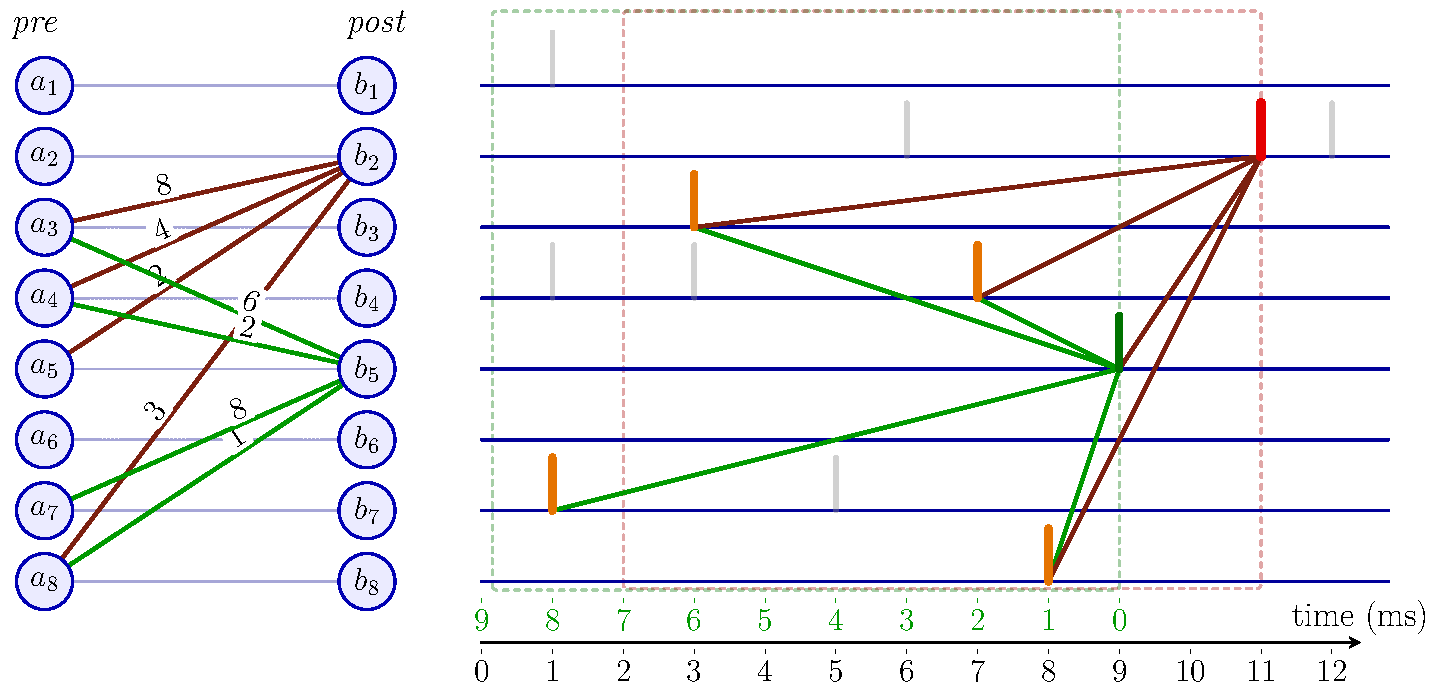
\includegraphics[width=\linewidth]{tikz_izhikevich.pdf}%
  % \end{adjustbox}
  \caption{%
    \textbf{Working memory as a chained sequential spike prediction via heterogeneous delays.}
    %
    \emph{Left:} A recurrent HD-SNN of eight neurons numbered $1$--$8$ for which two subsets of recurrent connections are shown that define two Spiking Motifs from the pre-synaptic side (denoted $a$) to the post-synaptic side ($b$): dark-red connections from $a_2$, $a_3$, $a_4$, and $a_5$ target $b_1$ with delays $3$, $8$, $4$, $2$\,ms; green connections from $a_2$, $a_3$, $a_4$, and $a_5$ target $b_5$ with delays $1$, $6$, $2$, $8$\,ms. %
    \emph{Right:} Raster plot of the same two motifs: each trajectory joins an input spike to the spike it contributes to, and faint grey spikes are from spontaneous activity.
    %
    \emph{Step~1, first prediction (green dashed box):} the orange input spikes emitted at staggered times by $a_2$--$a_5$ within the first context window (dashed green box) constitute a first Polychronous Group~\citep{Izhikevich2006}. As weights and delays can be tuned, this structure is called a Spiking Motif~\citep{Perrinet2023}. The green delays are tuned so that the four spikes, emitted at $t=8$, $3$, $7$ and $1$\,ms by $a_2$, $a_3$, $a_4$ and $a_5$, converge \emph{synchronously} at $b_5$ at $t=9$\,ms, crossing the firing threshold and producing the green output spike with a precise time.
    %
    \emph{Step~2, second prediction (dark-red dashed box):} the green spike of $b_5$ re-enters the population as a new input of $a_5$. Together with the spikes still visible in the shifted context window (dark-red dashed box), spikes are routed through the dark-red delays in order to converge synchronously on $b_1$ at $t=11$\,ms, generating a new output spike.
    %
    Because output spikes re-enter the same population, detecting one Spiking Motif provides the context for predicting the next spike in the sequence, implementing working memory as a chain of polychronous motifs in which each new temporal prediction is grounded in the preceding context window.
  }
  \label{fig:izhikevich}
\end{figure}
%%%-----------------------------------------------------------------

%----------------------------%
A century ago,~\citet{Adrian1926} established that neural communication relies on all-or-none action potentials, \emph{spikes}. Whether information is encoded in precise spike timing, for instance in coarsely synchronous activity with so-called \emph{synfire chains}, or in the coarser measure of instantaneous firing rate remains debated~\citep{Softky1993,Bohte2004,Grimaldi2023} --- a question that becomes especially sharp for working memory, where the brain must maintain and manipulate information across delays of seconds. In classical artificial neural networks, long-range temporal dependencies are addressed by gated recurrent unit (GRU) architectures or Transformers~\citep{Vaswani2017}, which decouple temporal binding range from the timescale of individual units. The analogous problem for spiking neural networks (SNNs) --- binding activity patterns separated by intervals far exceeding a single neuron's time constant --- lacks a general solution and remains a key challenge for biologically plausible sequence processing~\citep{Yin2026}.

\citet{Izhikevich2006} extended the synfire framework by introducing heterogeneous axonal delays in a recurrent population of spiking neurons trained with spike-timing-dependent plasticity (STDP). The resulting \emph{polychronous neuronal groups} (PNGs) --- time-locked, non-synchronous firing patterns at millisecond precision --- vastly outnumber the neurons in the network, yielding a large short-term memory capacity exploited for visual feature binding~\citep{Eguchi2018} and sequence classification~\citep{Paugam-Moisy2008}.~\citet{Szatmary2010} showed that short-term plasticity can cue a PNG's reactivation and sustain a working memory. However, storing spike patterns of arbitrary length is inherently difficult: the sequential structure of the task means each context window is not an independent query but is itself the output of the network at the previous step, so small errors at early time steps propagate and amplify towards the end of the sequence --- a compounding difficulty absent from static associative memory like Hopfield networks.

The limitation of the original model from~\citet{Izhikevich2006} is that delays are fixed rather than learned. Recent work addresses this:~\citet{Goltz2021} demonstrated fast, energy-efficient inference on neuromorphic hardware using first-spike-time coding, while~\citet{Hammouamri2023} introduced gradient-based delay learning via dilated convolutions with learnable spacings (DCLS), achieving sparse solutions in which only $\sim\!20\%$ of delay channels remain active. Applied to event-based vision, heterogeneous learned delays in a single spiking layer suffice for fast motion detection~\citep{Grimaldi2023a}, scalable to always-on object recognition~\citep{Grimaldi2024}. Building on this, \emph{Spiking Motifs} (SMs) generalise PNGs to a gradient-trainable, hardware-compatible framework by replacing fixed STDP rules with end-to-end learned delays, here referred to as Heterogeneous-Delay SNNs (HD-SNNs)~\citep{Perrinet2023}. However these motifs have a short time span equal to the range of possible delays, while it has been shown in mice stimulations that sequences of the order of seconds influence neural activity~\citep{Deveau2026}.~\citet{Kronland-Martinet2026} recently extended this to motifs of arbitrary length by chaining sub-motif detectors with bounded synaptic delays, achieving robust encoding of complete Spiking Heidelberg Digits patterns.

The present work extends the chain-of-motifs framework of~\citet{Kronland-Martinet2026} to a fully recurrent topology for working memory. Rather than relying on fixed delays and unsupervised STDP as in the original polychronisation model, the network is trained end-to-end with surrogate gradients~\citep{Neftci2019a}: once primed by a short trigger window of $D$ steps, it autonomously recalls arbitrary-length spike sequences, bridging polychronisation theory with gradient-based machine learning.

%%%-----------------------------------------------------------------
%%%-----------------------------------------------------------------
\section{Methods}
\label{sec:methods}
%%%-----------------------------------------------------------------
\subsection{Recurrent HD-SNN architecture} % MNESIS
%%%-----------------------------------------------------------------

In a previous work, we have demonstrated that a feedforward HD-SNN can learn to detect Spiking Motifs~\citep{Perrinet2023}. However, this architecture is limited to motifs of length $D$, the maximum synaptic delay. To store and recall longer sequences, it is possible to extend this architecture to a fully recurrent topology, where each neuron receives inputs from all other neurons across all delays. Our core concept is to retrieve a memory progressively, in which each motif of length $D$ would allow us to predict the next spikes in the memory to retrieve. This allows the network to generate a chain of overlapping Spiking Motifs, where each motif provides the context for predicting the next spikes in the sequence (see Figure~\ref{fig:izhikevich}).

In practice, we will study a recurrent Heterogeneous-Delay SNN (HD-SNN) which consists of a population $\mathcal{A}$ of $N = 1024$ leaky integrate-and-fire (LIF) neurons implemented in \texttt{snnTorch}~\citep{Eshraghian2023} and simulated over $T = 1000$ steps of $1\,\mathrm{ms}$ each (total duration: $1\,\mathrm{s}$). Extending the feedforward Spiking Motif Detector~\citep{Perrinet2023}, our architecture will include full recurrence: each neuron $j \in \mathcal{A}$  integrates inputs from \emph{all} other neurons across \emph{all} preceding $D = 41$ time steps. Such network is the most general for learning purposes, and at inference, pruning of the synapses may be added to gain from the sparseness of synapses on the energy budget. The choice for the maximum delay value $D$ is justified from biological observations and similar to the value used in the original polychronisation study~\citep{Izhikevich2006}. The membrane potential $u_j(t)$ evolves as
\begin{equation}
  u_j(t)
  = \beta \cdot u_j(t-1) \cdot (1 - s_j(t-1))
    + \sum_{i=1}^{N} \bigl (
      % b_i + 
      \sum_{d=1}^{D} \mathbf{W}_{j, i, d} \cdot s_i(t-d) \bigr ), 
  \label{eq:lif}
\end{equation}
where $\beta \in (0,1)$ is the membrane decay constant ($\beta = 0.7$ in our simulations, that is, a time constant of $\tau= 1 / \ln(\frac 1 \beta) \approx 2.8$ steps), $\mathbf{W}_{j, i, d}$ is the synaptic weight to neuron $j$ from neuron $i$ at delay $d$, and $s_j(t) \in \{0,1\}$  is the spike indicator $s_j(t) = \mathds{1}[u_j(t) \geq \vartheta]$, that is, $s_j(t)=0$ if $u_j(t) < \vartheta$ and a spike is emitted $s_j(t)=1$ when $u_j(t)$ exceeds the threshold $\vartheta$. After spiking, the membrane potential that is accumulated in Equation~\ref{eq:lif} is reset to zero.

In our implementation, the spike history of all $N$ neurons over the past $D$ steps is concatenated into a flattened context vector of dimension $N \cdot D$ at each time step, so that $\mathbf{W}$ is reshaped as $\mathbf{\bar W} \in \mathbb{R}^{N \times (N \cdot D)}$. This is equivalent to the temporal convolution that we used previously in a feedforward setting~\citep{Perrinet2023}, here extended to a fully recurrent topology. The HD-SNN thus maps onto a standard static computational graph that can be trained with surrogate gradient descent as classical SNNs (see Figure~\ref{fig:model}, left panel).

%%%-----------------------------------------------------------------
%!TeX encoding = UTF-8 Unicode
%!TeX spellcheck = en-UK
% !TeX root = Perrinet26mnesis.tex
% -*- coding: UTF-8; -*-
%%%-----------------------------------------------------------------
\begin{figure}%[htbp]
  \centering
  \adjustbox{valign=c,width=0.49\textwidth}{%
  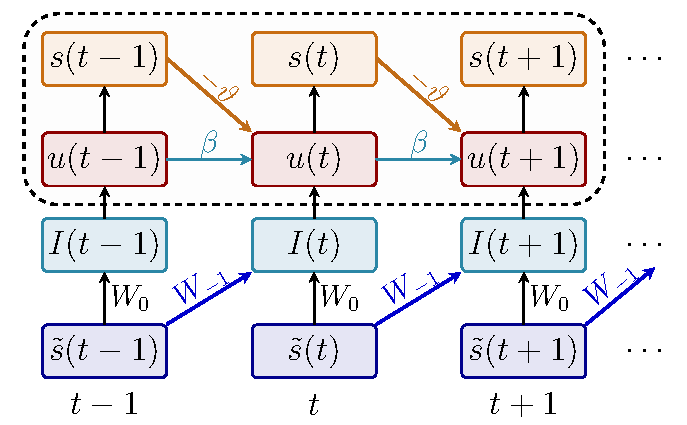
\includegraphics[width=\linewidth]{tikz_snntorch.pdf}%
  }
    \hfill
    \adjustbox{valign=c}{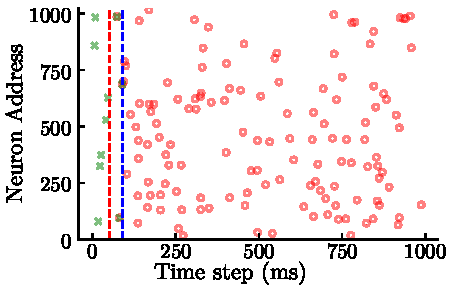
\includegraphics[width=0.49\textwidth]{pattern.pdf}}
  \caption{%
    Network architecture and a sample target motif. \emph{Left:}
    Unrolled view of the recurrent HD-SNN over time (one column representing one time step), illustrating delayed connections between neurons: Blue arrows indicate synaptic connections that integrate past activity across heterogeneous delays: the arrow labelled $\mathbf{W}$ stands for the weights over all $D$ delays. The context $\mathbf{c}(t)$ is the input received by the network at time $t$: the spike history over the $D$ previous steps, that is, the activity from $t-D$ to $t-1$ included ($t$ excluded), made of the target motif clamped during the trigger window, then the network's own recurrent spikes. Clamping input spikes is what excites the network: the trigger window is one such case, and other input spikes can be clamped in the same way. Once the trigger window is over, $\mathbf{c}(t)$ contains the spikes $s(t-1)$ emitted by the network itself, so that its output feeds back onto its input: this closes a recurrence loop, $s(t) \to \mathbf{c}(t+1) \to I(t+1) \to u(t+1) \to s(t+1)$, which the figure does not draw. The arrow labelled $-\vartheta$ depicts the subtractive reset of snnTorch, which subtracts the threshold from the membrane after each spike; the simulations reset the membrane to zero instead (Equation~\ref{eq:lif}), and the subtractive reset was one of the options scanned in Section~\ref{sec:hyperparameters}.
    \emph{Right:}
    One representative target spike motif, the second of the $M=16$ motifs, also shown in Figure~\ref{fig:target} ($N=1024$ neurons, $T=1000$ time steps); each red circle marks one target spike. The goal of the network is to memorise $M=16$ such motifs. Each trial is preceded by $50$ time steps of spontaneous background activity (random spikes at rate $p_A$) before the stimulus. The trigger window (green crosses between the dashed lines) consists of the first $D=41$ time steps of the target motif clamped to the network input; the recurrent network then autonomously predicts the remaining spikes.
  }\label{fig:model}
\end{figure}
%%%-----------------------------------------------------------------

%%%-----------------------------------------------------------------
\subsection{Synthetic dataset and definition of noise}
%%%-----------------------------------------------------------------
To assess working-memory capacity in all generality, we generated a dataset of $M = 16$ distinct target patterns $\mathbf{S}^{(\mu)} \in \{0,1\}^{N \times T}$. Following previous work~\citep{Perrinet2023}, each pattern is generated using a stochastic spiking pattern generator with both a structured and background component. Specifically, for each pattern we define a \emph{frozen} pattern as $P^{(\mu)} \in \{0,1\}^{N \times T}$ with $
  P^{(\mu)} \sim \mathrm{Bernoulli}(p_A)$ 
where we set $p_A = 1.6 \times 10^{-4}$ spike per neuron per time step ($0.16\,\mathrm{Hz}$ if we consider $1\,\mathrm{ms}$ time bins) as the average spike probability. This follows the estimation of the average spiking frequency in the human brain~\citep{Lennie2003}. 

To account for the stochasticity inherent to neural activity, we further include a balanced bit flipping mechanism with probability $p_\text{flip} = 0.01$. This is defined by the binary mask  $M^{(\mu)} \in \{0,1\}^{N \times T}$ of bit flips locations:
$
  M^{(\mu)} \sim \mathrm{Bernoulli}(p_\text{flip})
  $.
Values are left untouched where $M^{(\mu)} = 0$ and will be drawn with probability $p_A$ where $M^{(\mu)} = 1$. Finally, the spike patterns $S^{(\mu)} \in \{0,1\}^{N \times T}$ are those of the frozen pattern $P^{(\mu)}$ except where $M^{(\mu)} = 1$ for which they are obtained by drawing with probability $p_A$, that is $N^{(\mu)} \sim \mathrm{Bernoulli}(p_A)$. Formally, this can be expressed as:
\begin{equation}
  \mathbf{S}^{(\mu)} \sim P^{(\mu)} \cdot (1 - M^{(\mu)}) + N^{(\mu)} \cdot M^{(\mu)}
  \label{eq:pattern_generation}
\end{equation}
Note that the bit flipping mechanism introduces a stochasticity into the structure of the spike patterns, however, it does not change the average firing rate. Indeed, since the generation of $\mathbf{P}^{(\mu)}$ and $\mathbf{M}^{(\mu)}$ are independent, the expected firing rate $E(\mathbf{S}^{(\mu)})$ is equal to $p_A \cdot (1 - p_\text{flip}) + p_A \cdot p_\text{flip}= p_A$. 
%
%%%-----------------------------------------------------------------
\subsection{Working memory task: memory cuing}
\label{sec:task}
%%%-----------------------------------------------------------------
%
Given a set of target patterns as defined above, a generic working memory task consists of training the network to reproduce the target pattern that follow a short \emph{trigger} window. Formally, given $\mathbf{S}^{(\mu)}$, each contiguous window of length $D$, i.e.\ the slice $\mathbf{S}^{(\mu)}[\cdot,\, t{-}D:t{-}1]$, constitutes a unique context that may be used to predict the spiking activity $s_j(t)$ of all neurons $j$ at time $t$ (see Figure~\ref{fig:izhikevich}). The network is therefore trained to generate a sequential chain of overlapping Spiking Motifs~\citep{Perrinet2023,Kronland-Martinet2026} that faithfully reproduces the target. Memory retrieval is cued by clamping all neuron activities to the target pattern during the trigger window which corresponds to the initial $D$ time steps ($0 \le t < D$), that is, corresponding to one elementary Spiking Motif (see Figure~\ref{fig:model}, right panel); the goal of the network is then to generate the remainder of the sequence autonomously.

This chain of contexts has a structural weak point. A motif may contain a \emph{gap}, that is, a stretch of $D$ consecutive time steps in which none of the $N$ neurons fires. The context window that covers the gap is then empty, and since the synaptic current $I_j(t) = \sum_{i,d} \mathbf{W}_{j,i,d} \cdot s_i(t-d)$ has no bias term, it vanishes whatever the weights: no readout of the past $D$ steps can predict the spikes that follow the gap, and an autonomous replay necessarily stops at its onset. A given window is empty with probability $(1-p_A)^{N D} \approx e^{-p_A N D}$, that is $\approx 1.2 \times 10^{-3}$ for the default parameters ($p_A N D \approx 6.7$). Counting the gaps that open just after a time step containing at least one spike gives an expected number of $(T-D) \cdot (1 - e^{-p_A N}) \cdot e^{-p_A N D} \approx 0.18$ gaps per motif, so that about one motif in six is expected to contain at least one.

As an accuracy metric, we will use the $F_1$ score between the predicted spike trains and the frozen pattern $P^{(\mu)}$, whatever the realisation used to build the trigger, computed on the true and false positives and negatives pooled over time (in the prediction window), neurons and patterns. The $F_1$ score is the harmonic mean of precision (proportion of predicted activity that are correct) and recall (proportion of predicted activity that is successfully reproduced). Knowing a priori that average neural activity is sparse, minimising $\mathcal{L}$ simultaneously penalises over-active networks (low precision) and silent networks (low recall). 

Applied to the synthetic patterns, knowing $p_\text{flip}$ then one may first compute the precision as the ratio of expected true positives to the sum of true positives and false positives, that is, $\frac{p_A \cdot (1 - p_\text{flip} + p_A \cdot p_\text{flip})}{p_A \cdot (1 - p_\text{flip} + p_A \cdot p_\text{flip}) + p_\text{flip} \cdot (1 - p_A) \cdot p_A} = 1 - p_\text{flip} \cdot (1 - p_A)$. Then, recall is equal to precision as the average ratio of false negatives $p_A \cdot p_\text{flip} \cdot (1 - p_A)$ is equal to that of false positives (remember that the average frequency is not changed by the balanced bit flip operation). As a result, the average $F_1$ score between the frozen and perturbed patterns equals the precision and recall and is given by:
\begin{equation}
  F_1 = 1 - p_\text{flip} \cdot (1 - p_A)
  \label{eq:f1} 
\end{equation}
This value is the score of a noisy copy. It bounds the $F_1$ score that can be reached when the output is scored against a noisy realisation, as during training, since the flipped bits of a realisation cannot be predicted. It is not, however, a bound for retrieval, which is scored against the frozen pattern $P^{(\mu)}$: a network that has stored the frozen pattern itself, rather than one of its realisations, can replay it exactly from a noisy trigger window, and thus exceed this value (see Section~\ref{sec:results}).

%%%-----------------------------------------------------------------
\subsection{Analytical weight initialisation}
%%%-----------------------------------------------------------------
\label{sec:init}
From Equation~\ref{eq:lif}, by normalising the potential to arbitrary units, we wish the membrane potential to reach a sub-threshold value close to one whenever a spiking motif from a target pattern occurs. Before training, the weight tensor $\mathbf{W}$ can be initialised analytically by treating this task as a linear regression problem. For each target pattern $\mathbf{S}^{(\mu)} \in \{0,1\}^{N \times T}$, taken here as the frozen pattern $P^{(\mu)}$ (that is, with $p_\text{flip} = 0$), the context window at time $t$ is the flattened vector $\mathbf{c}^{(\mu)}(t) \in \{0,1\}^{N \cdot D}$ containing the spike history of all neurons over steps $t-D$ to $t-1$ and the corresponding desired output $\mathbf{I}(t) \in \{0,1\}^N$. Stacking all $K = M \cdot (T-D)$ context--output pairs across patterns and time steps yields
\[
  \mathbf{C} \in \{0,1\}^{(N \cdot D) \times K},
  \qquad
  \mathbf{I}^* \in \mathbb{R}^{N \times K},
\]
and the initialisation problem becomes $\mathbf{W}\,\mathbf{C} \approx \mathbf{I}$.

The choice of regression output $\mathbf{I}$ requires care. A naive choice is the binary spike matrix $\mathbf{S}$ itself, which would amount to ask the network to produce a current equal to the target spike at each step. However, the synaptic current $I_j(t) = \sum_{i,d} \mathbf{W}_{j,i,d} \cdot s_i(t-d)$ is not compared directly to $s(t)$: it is first \emph{filtered} by the membrane, which acts as a causal first-order IIR lowpass with transfer function $H(z) = 1/(1 - \beta \cdot z^{-1})$ and impulse response $h(t) = \beta^t$. The correct output is therefore obtained by deconvolution.  The inverse filter of $H(z)$ is $H^{-1}(z) = 1 - \beta \cdot z^{-1}$. Applied to a target trajectory that reaches $1$ at $t$ and resets immediately, the optimal input current is therefore
\begin{equation}
  I_j(t) \;=\; s_j(t) - \beta \cdot s_j(t-1).
  \label{eq:deconv_target}
\end{equation}
This is a \emph{biphasic} waveform: $1$ at each target spike time $t$ and $1-\beta$ exactly one step later, cancelling the residual membrane charge left by the leak. For $\beta \to 0$ the biphasic correction collapses to a scaled impulse; for $\beta = 0.7$ the negative lobe is substantial and significantly reduces spurious spikes.
 
Since the system is strongly underdetermined ($K \ll ND$), the minimum-$\ell_2$-norm solution is the Moore--Penrose pseudo-inverse $\mathbf{W}^* = \mathbf{I}^* \cdot \mathbf{C}^+$. With sparse neural activity at rate $p_A = 1.6\cdot 10^{-4}$, consecutive context windows are nearly orthogonal, so the Gram matrix of the contexts satisfies $\mathbf{C}^\top\mathbf{C} \approx N \cdot D \cdot p_A \cdot \mathbf{I}$, giving the closed-form initialisation
\begin{equation}
  w_{i, j, d}
  = \frac{1}{N \cdot D \cdot p_A}
    \sum_{\mu=1}^{M}\sum_{t=D+1}^{T}
    s_i^{*(\mu)}(t-d)
    \cdot
    \bigl(s_j^{*(\mu)}(t) - \beta \cdot s_j^{*(\mu)}(t-1)\bigr).
  \label{eq:init}
\end{equation}
Each weight $w_{i, j, d}$ is proportional to the cross-correlation between the deconvolved spike train of neuron $j$ and the raw spike train of neuron $i$ at delay $d$, summed over all $M$ patterns and normalised by the mean number $N \cdot D \cdot p_A$ of spikes in a context.

% TODO is it by definition low-rank ?

 We will set the threshold at $\vartheta = 0.75$ at each target spike time $t$, reserving a safety margin $\delta = 1 - \vartheta = 0.25$. This margin prevents spurious firings from partial contexts and, crucially, places the membrane in the regime where the surrogate gradient is near its maximum, making the first gradient step maximally informative.
  A perfect context thus drives the membrane to $u_j(t^*) = 1$, a margin $\delta = 0.25$ above the threshold, so that a context missing up to a quarter of its supporting spikes still evokes the target spike. This mirrors spike-timing-dependent plasticity (STDP)~\citep{Izhikevich2006} and classical Hebbian learning~\citep{Perrinet2002}, with the additional $-\beta$ correction accounting for the membrane leak. At inference time the network receives its own generated context rather than the ground truth, so errors can accumulate over time --- the primary source of difficulty analysed in Section~\ref{sec:results}.
%%%-----------------------------------------------------------------
\subsection{Training}
%%%-----------------------------------------------------------------
The loss is defined as $\mathcal{L} = 1 - F_1$, such that minimising this loss (with a maximum of $1$ and minimum of $0$) maximises the mean $F_1$ score across all $M$ target patterns. Learning is carried out with surrogate-gradient BPTT~\citep{Neftci2019a}, using a fast-sigmoid surrogate with sharpness parameter $\alpha = 5$. Weights are optimised with Adadelta, using a cosine learning-rate schedule with warmup, as used for instance in~\citep{Hammouamri2023}, from a base learning rate $\eta_\mathrm{base} = 40.0 \times 10^{-3}$ to a final learning rate $\eta_\mathrm{final} = 400 \times 10^{-6}$, with $16$ warmup epochs over $256$ total epochs. At each epoch, a new stochastic realisation of the patterns (Eq.~\ref{eq:pattern_generation}) is generated, acting as data augmentation. Dropout regularization with probability $0.60$ is applied to the post-synaptic current. The validation loss, computed for another realisation used as the trigger and scored against the frozen patterns $P^{(\mu)}$, is monitored for detecting overfitting; all realisations are drawn from explicit seeds, so that a run is reproducible.

The gradient-based learning in our recurrent HD-SNN shares fundamental principles with biological STDP, despite operating at different scales. Both mechanisms exploit temporal correlations in spike timing to adjust synaptic strengths. However, while STDP implements local pairwise updates based on individual spike timings, our approach performs global optimisation that effectively learns the collective interaction of multiple delayed spike trains across the entire network. The analytical initialisation (see Equation~\ref{eq:init}) reveals this connection most clearly: it implements a Hebbian-like rule that is mathematically equivalent to averaging STDP updates across all stored patterns, suggesting that gradient descent in this context can be viewed as a principled, globally optimal implementation of temporally structured synaptic plasticity.

Our implementation is available at \url{https://github.com/SpikeAI/MNESIS}. The recurrent HD-SNN was implemented using the snnTorch~\citep{Eshraghian2023} library with custom extensions for heterogeneous delay handling. The implementation leverages PyTorch with the Metal Performance Shader (MPS) backend for accelerated computation on Apple Silicon (M3 Ultra chip featuring 32 CPU cores and 80 GPU cores, with 512\,GB of unified memory architecture) and further tested with the CUDA backend on the Jean Zay supercluster at GENCI\@. The MPS and CUDA backends enabled efficient training and simulation of the large recurrent networks required for working memory tasks, leveraging the parallel processing capabilities of the GPU cores while maintaining low-latency access to the substantial memory resources necessary for storing all tensors' parameters. Training typically converged within $256$ gradient steps, requiring approximately $5$ minutes of computation time per training.
%
%%%----------------------------------------------------------------- 
\section{Results}
%%%----------------------------------------------------------------- 
\label{sec:results}
%%%----------------------------------------------------------------- 
\subsection{Training dynamics and results}
%%%----------------------------------------------------------------- 
%
We trained the recurrent HD-SNN with surrogate-gradient BPTT~\citep{Neftci2019a}, starting from the analytical initialisation, on $M=16$ target patterns with $N=1024$ neurons, $D=41$ delays, $T=1000$ time steps, $p_A=1.6\times10^{-4}$, and $\beta=0.7$ (time constant $\tau \approx 2.8\,\mathrm{ms}$). Without the analytical initialisation, two characteristic failure modes arise during early training: episodes of complete silence, in which the network emits no spikes, and over-activation, in which nearly all neurons fire at every time step. Both are well-known pathological attractors of recurrent SNNs~\citep{Izhikevich2006,Voges10jpp}. The $F_1$ score is the harmonic mean of precision and recall, and maximising it therefore penalises both failure modes symmetrically: low precision corresponds to an over-active network and low recall to a silent one. The cosine learning-rate schedule~\citep{Hammouamri2023} helped guide the network away from these extremes towards a balanced, sparse-firing regime. 

Remarkably, the analytical weight initialisation alone (Eq.~\ref{eq:init}) already achieves high $F_1$ scores before any gradient step, demonstrating that the closed-form Hebbian solution provides a strong baseline for recall on this benchmark. The Gram-matrix approximation $\mathbf{C}^\top\mathbf{C} \approx N \cdot D \cdot p_A \cdot \mathbf{I}$ reduces the pseudo-inverse to a simple cross-correlation (Eq.~\ref{eq:init}), but it does not preserve the accuracy. It assumes that every context contains the same number of spikes, whereas this number fluctuates around $N D p_A \approx 6.7$: with a normalisation by $N D p_A$, the sparsest contexts fall below threshold and the replay dies out ($F_1 \approx 0.12$ for the analytical initialisation), whereas a smaller normalisation makes it explode. The exact pseudo-inverse, whose weights adapt to the number of spikes of each context, is therefore used throughout ($F_1 \approx 0.80$); in the parameter scan, training from the approximation did not recover either ($F_1 \approx 0.001$, against $0.885$ with the pseudo-inverse). Gradient training, in contrast, left the replay unchanged. With the learning rates above, far below the nominal value of $1$ for Adadelta, the weights moved by at most $10^{-3}$ (a relative change of $2 \times 10^{-3}$ of their norm), whereas a perfect context exceeds the threshold by $\delta = 0.25$: not a single evoked spike changed, and the scores of the trained network were identical to those of the analytical initialisation, motif by motif and for each of $8$ realisations of the trigger window and of the spontaneous activity. The scores reported below are therefore those of the analytical solution, and their limits, analysed next, lie in the statistics of the motifs rather than in the optimisation.

The mean $F_1$ score, however, hides a strong heterogeneity between motifs, which we analysed for the analytical initialisation, cued by a noisy realisation of the trigger window ($p_\mathrm{flip} = 0.01$) preceded by $50$ steps of spontaneous activity. Scored motif by motif, $9$ of the $M = 16$ motifs were replayed exactly, without a single false positive or false negative ($F_1 = 1$). This exceeds the value $F_1 \approx 0.990$ of Equation~\ref{eq:f1} for a noisy copy: the replay restores the frozen motif, not the noisy realisation that provided the trigger window. The other motifs failed in one of two ways, which correspond to the two ends of the distribution of the number $K$ of spikes in a context window.

First, four motifs were replayed faithfully up to a given time step, after which their replay stopped (recall from $0.18$ to $0.56$). These are exactly the four motifs that contain a gap of $D$ silent steps ($K = 0$, Section~\ref{sec:task}), and for each of them the last correctly evoked spike immediately precedes the onset of the gap. This failure is structural rather than a defect of the weights: when the readout is fed with the exact history of the motif instead of the network's own spikes, the $F_1$ score of every motif, these four included, lies between $0.99$ and $1$, and these four motifs failed in the same way for each of $8$ realisations of the trigger window and of the spontaneous activity.

Second, four motifs (one of which also contains a gap) showed the opposite failure, an over-active replay (recall $1$ for the three motifs without a gap, precision from $0.46$ to $0.65$). Their false positives were not diffuse: all but $8$ of the $425$ false positives belonged to another stored motif, and the remaining ones to the same motif shifted in time, so that a second memory was replayed with a time shift alongside the correct one. As the readout is linear and the contexts nearly orthogonal, both chains coexist without disrupting each other. With the minimum-norm weights, each of the $K$ spikes that support a target spike carries a weight of about $1/K$, so that a context with few spikes ($K \le 3$ for $11\%$ of the contexts) can be completed by a handful of spurious spikes and ignite the corresponding motif. Such intrusions are seeded before the replay starts, while the network already runs on the spontaneous activity that precedes the trigger window: without this activity, only one intrusion remained. Which motifs suffer an intrusion therefore depends on the realisation. Over the $8$ realisations, the motif whose intrusion is driven by its trigger window alone was affected each time, whereas the other motifs without a gap had a degraded replay in $9$ of $88$ cases (all but one of them over-active), and the mean $F_1$ score ranged from $0.79$ to $0.84$ ($0.96$ when the four motifs with a gap are excluded). The gaps thus set a deterministic ceiling on the mean $F_1$ score, whereas intrusions make it vary from one realisation to the next.

%%%-----------------------------------------------------------------
%!TeX encoding = UTF-8 Unicode
%!TeX spellcheck = en-UK
% !TeX root = Perrinet26mnesis.tex
% -*- coding: UTF-8; -*-
%%%-----------------------------------------------------------------
\begin{figure}[!ht]
  \begin{center}
    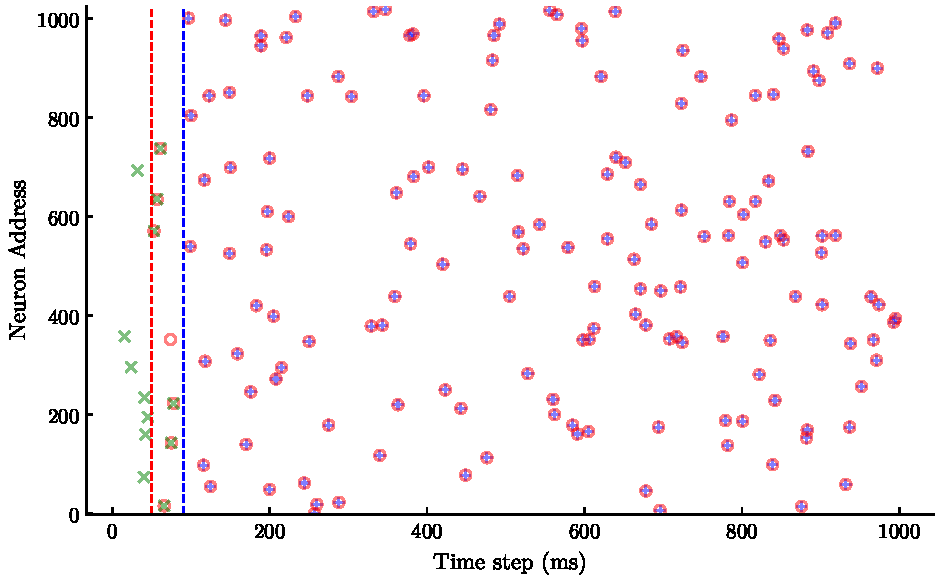
\includegraphics[width=\textwidth]{target.pdf}
  \end{center}
   \caption{Pattern retrieval by the recurrent HD-SNN after training. The network is clamped with input spikes (green crosses) comprising $50$ steps of spontaneous activity (left of the red dashed line) followed by the trigger window consisting of the initial sequence of one of the $M=16$ target motifs ($0 \leq t < D = 41$, delimited by the red and blue dashed lines). The motif shown, the second one, was chosen as characteristic of the average behaviour: with an intact trigger window, its $F_1$ score ($\approx 0.96$) is close to the median over the $M=16$ motifs ($\approx 0.95$). The autonomous replay is then simulated over the full sequence duration ($T = 1000$ steps). The raster plot shows network activity (blue plus signs, $N=1024$ neurons) which accurately matches the hidden target pattern which was cued during the trigger window. Note that the target spikes after the trigger window (red circles right of the blue dashed line) are hidden from the network.}\label{fig:target}
\end{figure}
%%%-----------------------------------------------------------------

%%%-----------------------------------------------------------------

%%%-----------------------------------------------------------------
\subsection{Effect of hyperparameters}
%%%-----------------------------------------------------------------
% 25_MNESIS_optuna.ipynb
We explored the learning hyperparameters jointly with a Bayesian optimisation (Optuna~\citep{Akiba2019}, multivariate tree-structured Parzen estimator) over $200$ trials of $128$ epochs each, that is, half of the production budget. Each trial sampled the optimiser, the LIF parameters ($\beta$, $\vartheta$, reset mechanism, and whether $\beta$ and $\vartheta$ are learnt), the surrogate sharpness $\alpha$, the learning-rate schedule and the dropout rate, and was scored by the loss $\mathcal{L} = 1 - F_1$ on a fresh realisation of the patterns. Parameter importances were estimated with fANOVA. Three parameters dominated, together accounting for $0.88$ of the total importance: the firing threshold $\vartheta$ ($0.52$), the optimiser ($0.20$) and the pseudo-inverse initialisation ($0.15$). We report their effect on the loss first, then that of the remaining parameters in decreasing order of importance.

\paragraph{Firing threshold $\vartheta$.}
The threshold was sampled log-uniformly over a factor $3.618$ around its default value, that is, in $[0.21, 2.7]$. Among the Adadelta trials, the median loss was $\mathcal{L} \approx 0.82$ for $\vartheta \le 0.4$, fell to between $0.14$ and $0.17$ for $0.5 < \vartheta \le 0.8$, rose slightly to between $0.19$ and $0.23$ for $0.8 < \vartheta \le 1$, and every one of the $24$ trials with $\vartheta > 1$ failed (median loss $1$, best loss $0.70$), whether or not $\vartheta$ was learnt. The best $10\%$ of trials all had $\vartheta \in [0.59, 0.78]$ (median $0.68$), a range that includes the default value $\vartheta = 0.75$. Both failure modes follow from the analytical initialisation (Section~\ref{sec:init}), which drives the membrane to $u = 1$ for a perfect context: above $\vartheta = 1$ the initialised network evokes almost no spike, and training did not recover from this silent state; well below it, the margin $\delta = 1 - \vartheta$ becomes so large that partial contexts and residual charges also cross the threshold, producing spurious spikes.

\paragraph{Optimiser.}
The importance of the optimiser reflects the failure of three of the five candidates rather than a fine ranking: Adam, AdamW and RMSprop reached a median loss $\mathcal{L} \approx 1$ (best losses $0.999$, $0.30$ and $0.999$ respectively), whereas Adadelta (median $0.26$, best $0.087$) and SGD with momentum (median $0.24$, best $0.16$) both learnt. Adadelta reached the lowest losses, and all of the best $10\%$ of trials used it. The momentum coefficients of the failing optimisers were however derived from the same search ranges as the decay rate of Adadelta, giving values above $0.989$ instead of the usual $0.9$, so that their failure may reflect this parameterisation rather than the optimisers themselves. Within Adadelta, the decay rate of the running averages (importance $0.04$) had no monotonic effect.

\paragraph{Pseudo-inverse initialisation.}
Replacing the pseudo-inverse $\mathbf{W}^* = \mathbf{I}^* \cdot \mathbf{C}^+$ by its Hebbian approximation (Equation~\ref{eq:init}) prevented learning: among the Adadelta trials, the median loss was $\approx 1$ with the Hebbian rule (best loss $0.62$) against $0.22$ with the pseudo-inverse (best loss $0.087$), and the best $10\%$ of trials all used the pseudo-inverse. With $N \cdot D \cdot p_A \approx 6.7$ active entries per context, the contexts are only approximately orthogonal, and the exact pseudo-inverse plausibly removes the crosstalk between overlapping contexts that the Hebbian rule neglects. By contrast, the deconvolution of the target (Equation~\ref{eq:deconv_target}) had a negligible importance ($0.001$): with the pseudo-inverse, the median loss was $0.22$ with and without it, suggesting that training compensates for the residual charge that the biphasic correction cancels at initialisation.

\paragraph{Learning rate.}
The importances of the base and final learning rates were modest ($0.01$ and $0.03$), but the best $10\%$ of trials concentrated in a narrow band, $\eta_\mathrm{base} \approx 19 \times 10^{-3}$ (90\% range $[12, 39] \times 10^{-3}$) and $\eta_\mathrm{final} \approx 1.0 \times 10^{-3}$ ($[0.54, 1.4] \times 10^{-3}$), within search ranges spanning a factor $3.618^2 \approx 13$ around the default values. Too small a rate was the main cause of failure: the trials in the lowest quartile of $\eta_\mathrm{base}$ ($\le 14 \times 10^{-3}$) or of $\eta_\mathrm{final}$ ($\le 0.56 \times 10^{-3}$) had a median loss close to $1$ ($F_1 \approx 0$), whereas the highest quartile of $\eta_\mathrm{final}$ reached the lowest median loss ($\mathcal{L} \approx 0.25$). As this search used half the production number of epochs, these optimal rates are not directly transferable to the production schedule ($\eta_\mathrm{base} = 40 \times 10^{-3}$ to $\eta_\mathrm{final} = 400 \times 10^{-6}$ over $256$ epochs).

\paragraph{Membrane decay $\beta$.}
The membrane decay, sampled uniformly in $[0, 1]$ (as an initial value when $\beta$ was also learnt), had a modest importance ($0.02$) but a consistent effect on the robustness of training. Among the Adadelta trials, the median loss increased from $\mathcal{L} \approx 0.21$ for $\beta \le 0.2$ to $\approx 0.56$ for $0.6 < \beta \le 0.8$ and $\approx 0.73$ for $\beta > 0.8$, while the best loss reached in each of these ranges stayed between $0.09$ and $0.11$ up to $\beta = 0.8$ (best trial: $\beta \approx 0.51$, $\mathcal{L} \approx 0.087$) and degraded to $0.24$ beyond. Accordingly, the best $10\%$ of trials all had $\beta \le 0.63$ (median $0.31$). A short membrane time constant thus makes learning more tolerant to the other hyperparameters, plausibly because the residual charge left by a partial context decays before it can trigger a spurious spike, whereas a well-tuned network still performs well up to $\beta \approx 0.8$. The default value $\beta = 0.7$ ($\tau \approx 2.8$ steps) lies within this range and keeps the biphasic correction of Equation~\ref{eq:deconv_target} significant.

\paragraph{Surrogate sharpness $\alpha$.}
Within the explored range ($\alpha$ from $1.4$ to $8.1$ in the sampled trials), the sharpness of the fast-sigmoid surrogate had a negligible importance ($0.002$). Among the Adadelta trials, the median loss stayed between $0.25$ and $0.33$ and the best loss between $0.09$ and $0.11$ for $\alpha$ from $1.4$ to $5$, and the best $10\%$ of trials spread over $\alpha \in [1.5, 3.1]$ (median $1.9$). Learning is thus robust to the choice of $\alpha$ in this range, which includes the default value $\alpha = 5$; larger values were sampled too rarely ($5$ trials) to be conclusive.

%%%-----------------------------------------------------------------
\subsection{Retrieval of multiple spike patterns}
%%%-----------------------------------------------------------------
%  this section reflects what is computed in 13_MNESIS_testing-inference.ipynb
%%%-----------------------------------------------------------------
%!TeX encoding = UTF-8 Unicode
%!TeX spellcheck = en-UK
% !TeX root = Perrinet26mnesis.tex
% -*- coding: UTF-8; -*-
%%%-----------------------------------------------------------------
\begin{figure}[!ht]
\begin{center}
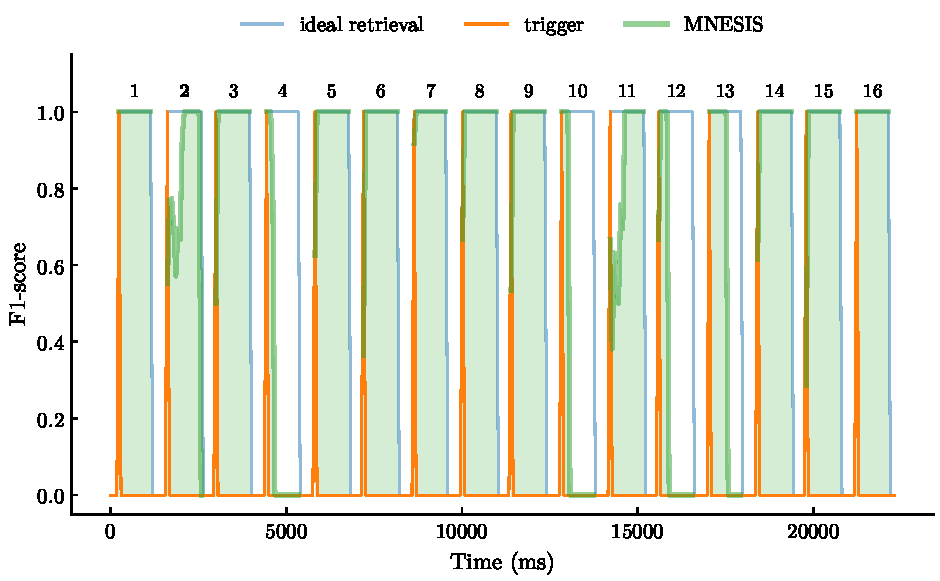
\includegraphics[width=\textwidth]{retrieval.pdf}
\end{center}
\caption{Sequential retrieval of the $M=16$ stored motifs. The motifs are concatenated into a single stream, each flanked on both sides by $200$ silent steps, and only their first $D=41$ steps are given to the network as a trigger. The $F_1$ score (green), computed in consecutive $60$-step windows against the frozen motifs, is shown over the duration of each motif (it is not shown in the silent intervals, where the target is empty), together with the trigger mask, equal to $1$ on each trigger window (orange), and the ideal retrieval envelope, equal to $1$ over the full $T=1000$-step duration of each motif (blue). The motifs are numbered above their envelope, and the number of the second one, shown in Figure~\ref{fig:target}, is in bold. Retrieval succeeds for $12$ of the $16$ motifs: the $F_1$ score rises at the trigger onset and stays close to $1$ until the end of the motif, in two cases (2nd and 11th motifs) after a partial dip that follows the trigger. For the 4th, 10th, 12th and 13th motifs, the replay starts correctly but breaks down after about $200$ to $600$ steps: the $F_1$ score then collapses to $0$ and does not recover before the end of the motif. Grey dashed lines indicate extremal $F_1$ values $0$ or $1$.}\label{fig:retrieval}
\end{figure}
%%%-----------------------------------------------------------------

%%%-----------------------------------------------------------------

Training was not uniform in time: the network first reproduced spikes immediately following the trigger window ($0 \leq t < D$), then progressively extended correct recall towards later time steps, as shown in Figure~\ref{fig:target}. This behaviour is a direct consequence of the sequential structure of the task: because each context window $[t-D,\, t-1]$ uniquely predicts the activity at time $t$, errors at early time steps propagate into all subsequent predictions, making temporal proximity to the trigger window the primary driver of learning progress.

To evaluate the network's ability to retrieve and distinguish multiple stored motifs in sequence, we concatenated all $M=16$ motifs into a single long raster, each trial flanked on both sides by $200$ silent steps, without spontaneous activity, so as to isolate trigger-driven retrieval (Figure~\ref{fig:retrieval}). Each motif was triggered by its individual trigger window, and retrieval was evaluated by the $F_1$ score in consecutive $60$-step windows, against the frozen motifs. For $12$ of the $16$ motifs, the $F_1$ score rose sharply at the onset of the trigger window and remained close to $1$ until the end of the motif (mean $F_1 \approx 0.96$ over these motifs): a single trigger window then suffices to select and replay the corresponding stored motif. For the four remaining motifs, the replay started correctly but broke down after about $200$ to $600$ steps, and the $F_1$ score then stayed at $0$ until the end of the motif, which brings the mean $F_1$ score over the $M=16$ motifs to $0.80$. This abrupt and irreversible failure is consistent with the chained structure of the replay: each spike is predicted from the preceding context window, so that once the activity deviates from the stored motif, the following context windows no longer correspond to it and the replay cannot recover (compare with the progressive extension of correct recall during training, Figure~\ref{fig:target}).

%%%-----------------------------------------------------------------
\subsection{Working memory and robustness to perturbations}
\label{sec:robustness}
%%%-----------------------------------------------------------------
%
A hallmark of biological working memory is graceful degradation: recall should remain possible under incomplete or corrupted retrieval cues, mirroring the tolerance of hippocampal pattern completion to partial input~\citep{Villette2015}. We therefore evaluated three distinct perturbations of the trigger window, each probing a different dimension of robustness (Figure~\ref{fig:noise}), and compared the $F_1$ score of the replay with a single model of its ignition, which has no fitted parameter.

%%%-----------------------------------------------------------------
%!TeX encoding = UTF-8 Unicode
%!TeX spellcheck = en-UK
% !TeX root = Perrinet26mnesis.tex
% -*- coding: UTF-8; -*-
%%%-----------------------------------------------------------------
\begin{figure}[!t]
\centering
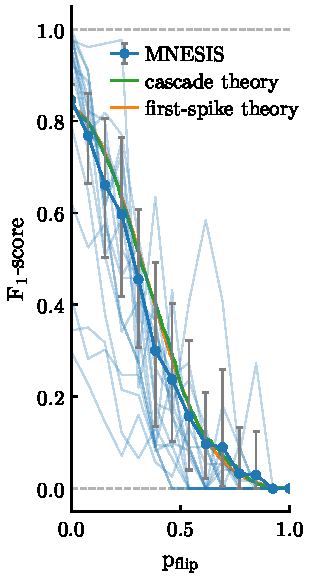
\includegraphics[width=0.333\linewidth]{p_flip_score.pdf}\hfill
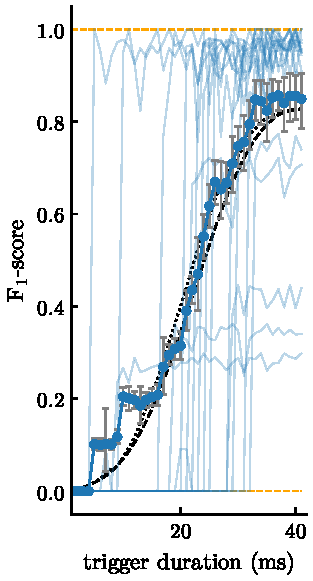
\includegraphics[width=0.333\linewidth]{trigger_time_score.pdf}\hfill
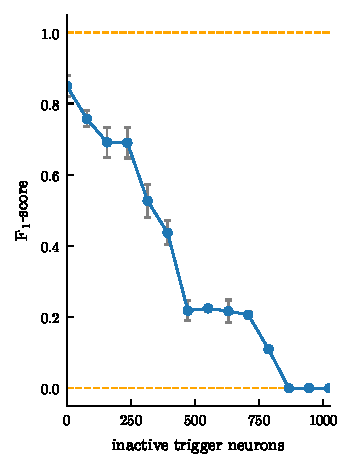
\includegraphics[width=0.333\linewidth]{fraction_target_score.pdf}
\caption{Robustness of working-memory retrieval to three types of trigger-window perturbation ($F_1$ score computed on the spikes of the $M=16$ patterns pooled together; a single trained network is cued by $11$ independent realisations of the perturbed trigger, each drawing the trigger noise and the spontaneous activity from its own random seed; each point is the mean over these realisations, and error bars span the $5\%$ to $95\%$ quantiles of a beta distribution fitted to them; thin blue lines show the $F_1$ score of each pattern, averaged over the realisations). \emph{Left:} Bit-flip noise applied to all spikes in the trigger window ($p_\mathrm{flip} \in [0,1]$); the network maintains high $F_1$ up to $p_\mathrm{flip} \approx 0.2$. \emph{Middle:} Truncated trigger window, reduced to its last steps (trigger duration from $1$ to $D = 41$ steps); retrieval remains reliable for durations above roughly $29$ steps. \emph{Right:} Partial neuron coverage (number of silenced neurons from $0$ to $N = 1024$); the $F_1$ score degrades smoothly as more neurons are silenced and drops sharply once the majority of the trigger population is inactive. In each panel, the dashed black line is the $F_1$ score expected from an ignition model, in which the replay of a pattern, a cascade decided by its first evoked spike, starts only if at least a fraction $\vartheta$ of the $\approx p_A N D \approx 6.7$ spikes supporting that spike are present in the perturbed trigger window (a mean-field model of the pseudo-inverse readout, with the precision and recall of the intact trigger as its only measured inputs); the dotted black line simulates the whole cascade. Orange dashed lines indicate extremal $F_1$ values $0$ or $1$.}\label{fig:noise}
\end{figure}
%%%-----------------------------------------------------------------
%%%-----------------------------------------------------------------
\paragraph{Replay as a cascade.}
Retrieval is not a one-shot completion of the trigger window but a cascade. At each step, a neuron fires when its context, the spikes of all neurons over the last $D$ steps, matches a context in which it fired during training (Section~\ref{sec:task}). During the trigger window, this context is imposed from outside; after it, the context is made more and more of the network's own output, and entirely so after $D$ steps. Each emitted spike thus joins the context of the next ones: a correct spike makes the next spikes of its pattern more likely, and a missed one makes them less likely. This positive feedback loop has two stable states. Either the evoked spikes complete the contexts of the next ones, and the replay ignites and sustains itself over the whole pattern, the noise-free pattern being a stable fixed point of the recurrent dynamics; or they fall short, the contexts of the next spikes keep shrinking, and the replay dies out. A perturbation of the trigger window therefore does not degrade the replay gradually: it decides, pattern by pattern, which of the two states is reached, and the $F_1$ score measures the fraction of patterns that ignite. Two observations support this picture. First, for the deterministic perturbations, the truncation of the trigger window and the lesion of a fixed set of neurons, the $F_1$ score of each pattern (thin lines in Figure~\ref{fig:noise}) switches abruptly between zero and its intact value, each pattern at its own level of perturbation; under random flips, where it is averaged over the realisations of the noise, it decays smoothly, as the probability that the pattern ignites. Second, in an open-loop control in which the output spikes are not fed back to the network, the trigger window alone drives the first $D$ steps after it, after which the activity vanishes: the replay is sustained by the recurrent feedback, not by the trigger.

\paragraph{Ignition model.}
A mean-field model of the analytical initialisation (Equation~\ref{eq:init}) makes this cascade quantitative. The minimum-norm solution gives equal weights to the $K$ spikes of a pattern that lie in the $D$ steps before one of its spikes, so that the membrane potential reaches $1$ when all of them are present and $k/K$ when only $k$ of them are, while a spurious spike of the trigger window falls on a near-zero weight, the patterns being sparse; the spike is thus emitted if $k \geq \lceil \vartheta K \rceil$. As the first evoked spike of a pattern sets off or not the positive feedback loop, it decides the fate of the replay. A pattern emits $\nu = p_A N \approx 0.16$ spikes per step, so that this spike occurs $\Delta$ steps after the trigger window with probability $P(\Delta) = e^{-\nu \Delta}(1 - e^{-\nu})$, and its context, made of the last $D - \Delta$ steps of the trigger window, holds a Poisson number $K$ of spikes of mean $\lambda_\Delta = \nu (D - \Delta)$, that is, $p_A N D \approx 6.7$ for $\Delta = 0$. When each of these spikes is present in the perturbed trigger window with probability $q_\Delta$, the replay of a pattern ignites with probability
\begin{equation}
  R = \frac{1}{R_0} \sum_{\Delta=0}^{D-1} P(\Delta) \sum_{K \geq 1} \frac{e^{-\lambda_\Delta} \lambda_\Delta^K}{K!} \sum_{k = \lceil \vartheta K \rceil}^{K} \binom{K}{k}\, q_\Delta^k \, (1 - q_\Delta)^{K - k},
  \label{eq:ignition}
\end{equation}
where $R_0 \approx 0.991$ is its value for the intact trigger window ($q_\Delta = 1$): the remaining failures are those of the patterns whose first evoked spike follows a gap (Section~\ref{sec:task}), already counted in the recall of the intact trigger. An ignited pattern is replayed with the precision $\pi_0$ and recall $r_0$ measured with the intact trigger window, and a silent one only adds false negatives, so that $F_1 = 2 R\, r_0 / (1 + R\, r_0 / \pi_0)$ (dashed lines in Figure~\ref{fig:noise}). The three perturbations differ only by the presence probability $q_\Delta$. To check that the first step decides the cascade, we also simulated the whole cascade on $2000$ random patterns of the same statistics, the emitted spikes joining the context of the next ones (dotted lines in Figure~\ref{fig:noise}).

\paragraph{Robustness to spike noise (Figure~\ref{fig:noise}, left).}
% 14_MNESIS_testing-noise.ipynb
We corrupted the trigger window with the balanced bit flips of Equation~\ref{eq:pattern_generation}, each bin being redrawn with probability $p_\mathrm{flip} \in [0, 1]$, and scored the replay against the frozen pattern. At $p_\mathrm{flip} = 0.25$, the network still achieved an $F_1$ score of $\approx 0.627$ (precision $\approx 0.898$, recall $\approx 0.481$), demonstrating a reasonable tolerance to noise in the trigger window. The $F_1$ score decreases monotonically as $p_\mathrm{flip}$ increases, reaching chance level only near $p_\mathrm{flip} = 0.5$, although the trigger window is entirely randomised only at $p_\mathrm{flip} = 1$. A spike of the trigger window survives the flips with probability $q_\Delta = 1 - p_\mathrm{flip}(1 - p_A)$, whatever $\Delta$, and Equation~\ref{eq:ignition} captures this decay; the simulated cascade gives the same curve, which confirms that the first evoked spike decides the replay. Each pattern has its own sensitivity to the flips (thin lines), as expected from the variability, from one pattern to the next, of the number of spikes that support its first evoked spike. This behaviour is consistent with the network operating as an attractor: small perturbations of the initial state are corrected by the recurrent dynamics, which converge back to the stored pattern.

\paragraph{Robustness to trigger-window duration (Figure~\ref{fig:noise}, middle).}
% 15_MNESIS_testing-trigger-duration.ipynb
% TODO: the numbers of this paragraph come from a run made before 2026-10-26, when the trigger kept the first steps of the window; update them after the rerun
We reduced the trigger window to its last $L$ steps, the first $D - L$ steps carrying spontaneous activity, with a duration $L$ from $1$ to $D = 41$ steps, scanning from a single step of cue to the full trigger window. At $75\%$ of the full trigger duration ($\approx 30$ steps out of $D = 41$), the network achieved an $F_1$ score of $\approx 0.416$ (precision $\approx 0.632$, recall $\approx 0.310$). The $F_1$ score increases monotonically with trigger duration, rising steeply once the trigger exceeds roughly $D/2$. The truncated trigger keeps the most recent part of the window, where the context of the first evoked spike lies: a spike of this context is present with probability
\begin{equation*}
  q_\Delta = \frac{\min(L, D - \Delta)}{D - \Delta} \, \big(1 - p_\mathrm{flip}(1 - p_A)\big),
\end{equation*}
larger than the share $L / D$ of the window, and Equation~\ref{eq:ignition} predicts the rise (dashed line in Figure~\ref{fig:noise}, middle). Unlike the two other perturbations, later evoked spikes, whose context is even more recent, give a pattern a few more chances to ignite when the first one fails, so that the simulated cascade lies slightly above the model (dotted line).

\paragraph{Robustness to partial neuron coverage (Figure~\ref{fig:noise}, right).}
% 16_MNESIS_testing-trigger-fraction.ipynb
We varied the number of neurons whose activity was silenced during the trigger window, from $0$ (full trigger) to $N = 1024$ (no trigger). With $N/8 = 128$ neurons silenced --- meaning $87.5\%$ of the population remained active --- the network still achieved an $F_1$ score of $\approx 0.602$ (precision $\approx 0.837$, recall $\approx 0.469$). The $F_1$ score degrades smoothly as more neurons are silenced and drops sharply only when the majority of the trigger population is inactive, again consistent with an attractor interpretation in which a sufficient fraction of the pattern suffices to pull the network dynamics towards the stored memory. Silencing $n$ neurons removes the same fraction of every part of the window, so that $q_\Delta = (1 - n/N)\big(1 - p_\mathrm{flip}(1 - p_A)\big)$ whatever $\Delta$, and Equation~\ref{eq:ignition} predicts this decay (dashed line in Figure~\ref{fig:noise}, right), as does the simulated cascade (dotted line); the plateau at $F_1 \approx 0.2$ that lies above it beyond $n \approx N/2$ is a finite-size effect, as the lesion always silences the same addresses and the two of the $M = 16$ patterns whose trigger spikes fall mostly on the remaining neurons keep igniting.
%
%%%-----------------------------------------------------------------
\subsection{Effect of delay depth, pattern duration, network size, and firing rate}
%%%-----------------------------------------------------------------
%  20_MNESIS_scanning-parameters.ipynb

To characterise how the architectural parameters govern working-memory performance, we conducted a systematic one-at-a-time scan over the maximum delay $D$, the pattern duration $T$, the number of neurons $N$, and the average firing probability $p_A$, holding all other hyperparameters at their default values (Section~\ref{sec:methods}). Each condition was evaluated with $10$ independent runs (random seeds) and results are reported as the mean $F_1$ score (Section~\ref{sec:task}) of the evoked window (Figure~\ref{fig:scan}).

%%%-----------------------------------------------------------------
%!TeX encoding = UTF-8 Unicode
%!TeX spellcheck = en-UK
% !TeX root = Perrinet26mnesis.tex
% -*- coding: UTF-8; -*-
%%%-----------------------------------------------------------------
\begin{figure}[!t] 
  \centering
  % the panels are printed at fig_width/3 by notebook 20, hence scaled by 3/4 here: use fig_width/4 at its next run
  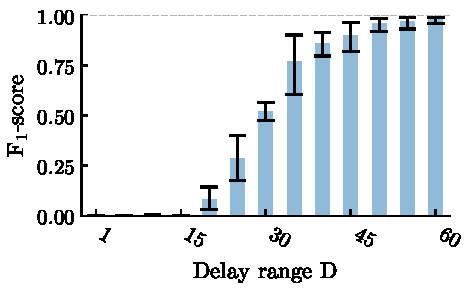
\includegraphics[width=0.25\linewidth]{scan_num_delay.pdf}\hfill
  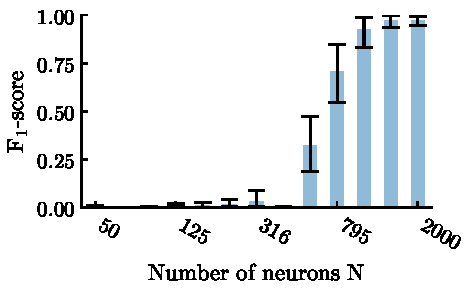
\includegraphics[width=0.25\linewidth]{scan_N_neuron.pdf}\hfill
  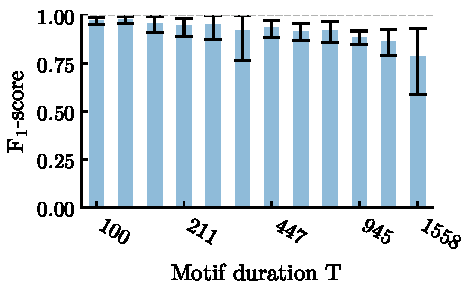
\includegraphics[width=0.25\linewidth]{scan_N_time.pdf}\hfill
  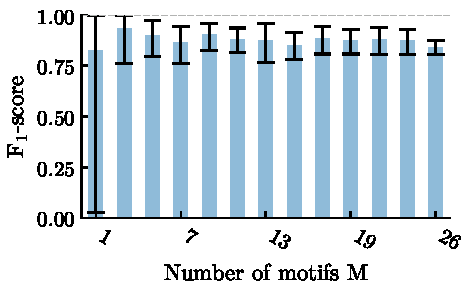
\includegraphics[width=0.25\linewidth]{scan_N_pattern.pdf}
  % TODO 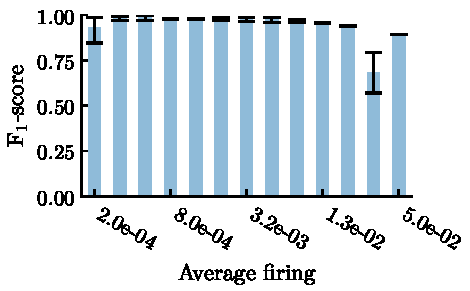
\includegraphics[width=0.9\linewidth]{scan_p_A.pdf}
  \caption{%
    Effect of some key parameters on working-memory performance ($F_1$ score over $10$ independent runs, each training a new network on new patterns drawn from its own random seed, a given seed sharing its patterns across all values of a parameter; bars show the mean over these runs, and whiskers span the $5\%$ to $95\%$ quantiles of a beta distribution fitted to them). %
    \emph{From left to right:}
    The $F_1$ score rises steeply with the maximum delay $D$ and with the number of neurons $N$: both increase the mean number $p_A N D$ of spikes in a context window, and thus decrease the probability that a motif contains a gap of $D$ silent steps, at which its replay stops. %
    It decreases slowly with the pattern duration $T$, as a longer motif is more likely to contain such a gap. %
    It does not depend on the number of stored motifs $M$ over the scanned range, up to $M = 26$.
  }\label{fig:scan}
\end{figure}
%%%-----------------------------------------------------------------

%%%-----------------------------------------------------------------
\paragraph{Delay depth $D$ (Figure~\ref{fig:scan}, left).}
The $F_1$ score increases monotonically as $D$ grows from $3$ to $127\,\mathrm{ms}$, rising from $F_1 \approx 0.15$ at $D = 3$ to near one at $D = 127$. This confirms the capacity argument: the parameter budget $N^2 \cdot D$ and the context-window size $N \cdot D$ both scale linearly with $D$. A wider delay window provides more temporally diverse synaptic pathways, increasing the number of simultaneously representable Spiking Motifs and reducing interference between overlapping context windows. At $D = 3$ the context vector has only $N \cdot D = 3072$ dimensions with expected activity $N \cdot D \cdot p_A \approx 3.07$ --- a regime where contexts are nearly all-zero and indistinguishable. At $D = 127$ the context has $N \cdot D = 129{,}024$ dimensions with expected activity $\approx 129$, and near-orthogonality is strongly satisfied.

\paragraph{Pattern duration $T$ (Figure~\ref{fig:scan}, middle).}
The $F_1$ score decreases slowly and monotonically with $T$, from $F_1 \approx 0.996$ at $T = 64$ to $F_1 \approx 0.92$ at $T = 2048$. This is the empirical signature of the two compounding difficulties identified in the capacity analysis: longer sequences impose a larger open-loop rollout, and the error propagation recurrence accumulates over $T - D$ steps. Even a sub-critical propagation coefficient $\lambda < 1/D$ eventually allows errors to reach a non-negligible fraction of $N$ spikes.

\paragraph{Network size $N$ (Figure~\ref{fig:scan}, right).}
The $F_1$ score remains close to zero for populations below about $400$ neurons, then rises steeply between $N \approx 500$ and $N \approx 1000$, and stays high ($F_1 \gtrsim 0.9$) from $N \approx 1000$ onwards. This threshold behaviour follows from the orthogonality argument: at fixed $D = 41$ and $p_A = 1.6 \times 10^{-4}$, the expected number of active entries in a context window, $N \cdot D \cdot p_A$, falls from $\approx 6.7$ at $N = 1024$ to $\approx 2.6$ at $N = 400$, too few for successive contexts to be reliably distinguished.

\paragraph{Firing rate $p_A$.}
We scanned the average spike probability from $p_A = 2 \times 10^{-4}$ to $5 \times 10^{-2}$ per neuron and per step ($0.2$ to $50\,\mathrm{Hz}$). The $F_1$ score stayed high ($\approx 0.98$) from $p_A \approx 3 \times 10^{-4}$ to $1.3 \times 10^{-3}$, then decreased slowly to $\approx 0.94$ at $p_A = 2 \times 10^{-2}$ and dropped to $\approx 0.70$ at $p_A \approx 3 \times 10^{-2}$ (with a non-monotonic $F_1 \approx 0.89$ at the largest rate), confirming that sparse activity facilitates stable recurrent dynamics~\citep{Izhikevich2006,Yin2026}. Higher firing rates increase the overlap between the contexts of different patterns, and thus inter-pattern interference, echoing the capacity bounds reported for polychronous neuronal groups~\citep{Szatmary2010}. Conversely, at the lowest rate ($p_A = 2 \times 10^{-4}$), the score was lower and more variable ($F_1 \approx 0.92$), as a context then contains only $N \cdot D \cdot p_A \approx 8$ active entries on average.

Taken together, the  scans quantitatively validate the theoretical framework: delay depth is the primary capacity lever (error $1 - F_1 \propto 1/(N \cdot D \cdot p_A)$), pattern duration is the primary difficulty lever, and the population must exceed a minimal size for contexts to be orthogonal enough for initialisation and learning to converge. These results suggest that the most efficient path to storing longer patterns is to increase $D$ rather than $N$, since $D$ enters both the parameter capacity $N^2 \cdot D$ and the context orthogonality $N \cdot D \cdot p_A$ while adding no new neurons or lateral connections. Increasing $D$ is, however, ultimately limited by biological constraints on axonal conduction delays~\citep{Grimaldi2023a}.

% not in ICANN :
%%%-----------------------------------------------------------------
\subsection{Retrieval of periodic spike patterns}
\label{sec:periodic}
%%%-----------------------------------------------------------------
%  this section reflects what is computed in 18_MNESIS_learn-periodic.ipynb

The working memory task above has a natural end: once the last context window of a motif has been replayed, nothing in the stored chain predicts further activity, and the network falls silent. A simple modification of the motifs turns this finite chain into an endless one. For each frozen motif, we copied its trigger window onto its last $D$ time steps, that is, $P^{(\mu)}[\cdot,\, T-D+t] = P^{(\mu)}[\cdot,\, t]$ for $0 \le t < D$, the same wrap being applied to each noisy realisation after the bit flips of Equation~\ref{eq:pattern_generation}. The last context window of a motif is then identical to its trigger window, so that a faithful replay of the end of the motif re-cues its beginning: the chain of overlapping Spiking Motifs closes on itself, with a period of $T - D = 959$ steps. The network was trained exactly as in the main experiment, with the same parameters and on a single period of $T = 1000$ steps, so that it never experienced the transition from one period to the next during learning. Cued by a noisy realisation of the trigger window ($p_\mathrm{flip} = 0.01$), the replay of the first period reached an $F_1$ score of $\approx 0.850$ (precision $\approx 0.875$, recall $\approx 0.827$).

We then cued the network with the noise-free trigger window and let it run freely for $30$ periods ($28\,770$ steps, about $29\,\mathrm{s}$), scoring each period separately against the frozen motif. The first period reached an $F_1$ score of $\approx 0.880$ (precision $\approx 0.940$, recall $\approx 0.827$), and from the second period onwards the score stayed at $\approx 0.829$ (precision $\approx 0.934$, recall $\approx 0.746$) without any further decline. The evoked rasters were in fact strictly identical from one period to the next: the network settled into an exact limit cycle. The drop in recall between the first two periods reflects an all-or-none selection at the first closure of the cycle. For $12$ of the $M = 16$ motifs, the replay reached the end of the motif and re-cued itself, after which it was sustained indefinitely; for the $4$ remaining motifs, the replay had already faded within the first period (from $28$ to $92$ evoked spikes) and these motifs stayed silent afterwards. These $4$ motifs are precisely those that contain a gap of $D$ silent steps (Section~\ref{sec:task}), which the wrap leaves untouched: their replay stops at the onset of the gap, whatever the trigger, and cannot reach the end of the motif to re-cue its beginning. The stationarity of the score follows from deterministic recurrent dynamics: once the activity over the last $D$ steps of a period matches that of the previous period, the next period is replayed identically. As a consequence, errors do not accumulate from one period to the next; they are settled once and for all during the first period.

Finally, we combined this long-horizon replay with the trigger-window noise of Section~\ref{sec:robustness}: the trigger window was corrupted by balanced bit flips with $p_\mathrm{flip} \in [0, 1]$ ($14$ levels), after which the network ran freely for $100$ periods, each period being scored against the frozen motif (Figure~\ref{fig:periodic}); each noise level was evaluated on a single seeded realisation of the corrupted trigger. At every noise level, the score reached a stationary value at the latest from the second period onwards, and kept it up to the hundredth period: the limit cycle is reached whatever the perturbation, which only determines how much of the motifs it retains. With an uncorrupted trigger ($p_\mathrm{flip} = 0$), the $F_1$ score went from $\approx 0.850$ in the first period to $\approx 0.801$ in the stationary regime, slightly below the previous run, from which this one differs only by the realisation of the spontaneous activity preceding the trigger window. The stationary score decreased with the noise level, to $\approx 0.60$ at $p_\mathrm{flip} \approx 0.23$ and $\approx 0.45$ at $p_\mathrm{flip} \approx 0.31$, then lay between $0.21$ and $0.26$ for $p_\mathrm{flip}$ from $0.38$ to $0.54$ and below $0.1$ beyond $p_\mathrm{flip} \approx 0.6$, with no sustained replay at all from $p_\mathrm{flip} \approx 0.85$. This decay is comparable to that of the replay of non-periodic motifs (Figure~\ref{fig:noise}, left), up to small non-monotonic variations due to the single realisation per level. The perturbation of the trigger window is thus filtered during the first period, after which a periodic memory is either sustained or lost, but never degraded further.

%%%-----------------------------------------------------------------
%!TeX encoding = UTF-8 Unicode
%!TeX spellcheck = en-UK
% !TeX root = Perrinet26mnesis.tex
% -*- coding: UTF-8; -*-
%%%-----------------------------------------------------------------
\begin{figure}[!t]
\centering
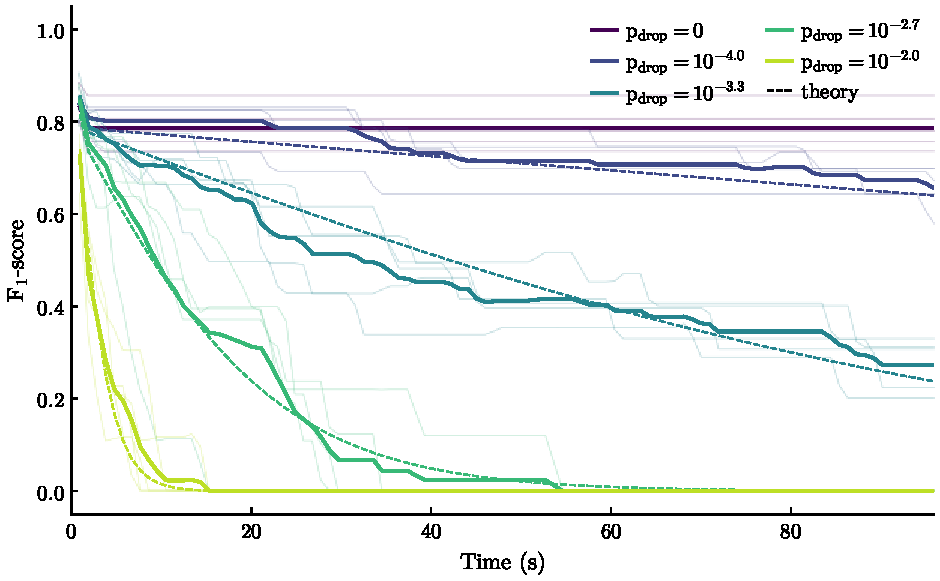
\includegraphics[width=\linewidth]{periodic_scores.pdf}
\caption{Free replay of periodic motifs under transmission failures. The motifs are made periodic by copying their trigger window (the first $D=41$ steps) onto their last $D$ steps, so that the chain of Spiking Motifs closes on itself with a period of $T-D=959$ steps of $1\,\mathrm{ms}$, that is $0.959\,\mathrm{s}$, about one second. After a single noisy trigger window ($p_\mathrm{flip} = 0.01$), each spike emitted by the network is removed from the recurrent input with probability $p_\mathrm{drop}$, and the network runs freely for $100$ periods ($95.9\,\mathrm{s}$). Each curve is one level of $p_\mathrm{drop}$, as given by the legend: $p_\mathrm{drop} = 0$ and four log-spaced levels from $10^{-4}$ to $10^{-2}$. Thin lines show the $5$ seeded realisations of each level, thick lines their mean. Each period is scored ($F_1$ score computed on the spikes of the $M=16$ motifs pooled together) against the frozen motif, and plotted at the time at which the period ends, counted from the end of the trigger window. Dashed lines: prediction of the cascade model (Section~\ref{sec:robustness}), in which each spike of a sustained replay is a new ignition test, so that the replay survives $t$ steps with probability $\exp(-ht)$. Without failures, the score settles on the limit cycle after the first period; with failures, the replay decays with a mean lifetime $1/(hP)$ of about $280$, $60$, $12$ and $2$ periods at the four non-zero levels.}\label{fig:periodic}
\end{figure}
%%%-----------------------------------------------------------------

%%%-----------------------------------------------------------------


%%%----------------------------------------------------------------- 
\section{Discussion}
%%%-----------------------------------------------------------------

\subsection{Memory capacity and the role of heterogeneous delays}
%%%-----------------------------------------------------------------

We have demonstrated that a recurrent SNN with heterogeneous synaptic delays can store and reproduce arbitrary target spike patterns, with the analytical weight initialisation providing a strong starting point for recall on a benchmark of $M=16$ patterns of $T=1000$ steps. The result is noteworthy from a capacity standpoint: the entire network is parameterised by a single weight tensor $\mathbf{W} \in \mathbb{R}^{N \times N \times D}$ of dimension $N^2 \cdot D = 1024^2 \cdot 41 \approx 43 \times 10^6$ parameters, yet it faithfully stores $M$ patterns each of $N \cdot T$ binary values. This compression is made possible precisely by the temporal structure introduced by the $D$ delay channels: rather than requiring one parameter per stored bit, the network exploits the sequential dependencies between consecutive context windows of length $D$ to represent the entire pattern as a chain of overlapping Spiking Motifs~\citep{Perrinet2023,Kronland-Martinet2026}. The memory limit is determined by parameter count rather than interference --- the marginal parameter cost per additional stored pattern is zero, and the capacity scales as $N^2 \cdot D$, linear in the delay depth. This provides concrete evidence that heterogeneous delays are a computational asset rather than a biological nuisance, a point argued theoretically in~\citet{Izhikevich2006} and demonstrated empirically in the context of learnable delays in feedforward~\citep{Grimaldi2023a,Hammouamri2023} and recurrent architectures~\citep{Queant2025,Meszaros2025}, and which we extend here to a full working-memory setting.

% TODO importance of sparse coding~\citep{Perrinet2002image}

% TODO make an analogy with mamba

The robustness experiments further strengthen this interpretation. Retrieval remains well above chance with $25\%$ bit-flip noise in the trigger window ($F_1 \approx 0.63$), becomes reliable once the trigger exceeds roughly $32$ of its $D = 41$ steps, and still reaches $F_1 \approx 0.60$ when $128$ of the $N = 1024$ trigger neurons ($12.5\%$) are silenced. This progressive degradation profile is consistent with the network operating as an attractor: the stored patterns correspond to stable fixed points of the recurrent dynamics, and the trigger window provides a partial cue that the network completes autonomously; the ignition model shows that this completion is a cascade, a positive feedback loop decided pattern by pattern by the few trigger spikes that support the first evoked spike, and the open-loop control shows that the replay is then sustained by the recurrent feedback rather than by the trigger --- the same mechanism proposed for hippocampal pattern completion~\citep{Villette2015}.

\subsection{Limitations and directions for improvement}
%%%-----------------------------------------------------------------

The present model is deliberately minimal, and several design choices impose limits on capacity and robustness that future work should address.

\paragraph{Capacity and scaling.}
A systematic evaluation of memory capacity --- how many patterns of what duration can be reliably stored and retrieved --- remains to be carried out beyond the present $M=16$ benchmark. The theoretical analysis predicts that capacity scales as $N^2 \cdot D / (T-D)$, giving approximately $5{,}700$ patterns for the current architecture, but whether gradient-based training reliably reaches this bound at scale is an open empirical question, as the implementation does not scale well with respect to the size of the GPU's memory. Interference between stored patterns at high memory load may degrade precision in ways that the F1 training objective does not fully penalise, and the sensitivity of recall to perturbations of the trigger window is expected to decrease as $M$ grows.

\paragraph{Richer neuron models and dynamics.}
We used the simplest LIF model with a fixed membrane decay $\beta$. Introducing adaptive threshold dynamics or more complex single-neuron models, as studied in~\citet{Szatmary2010}, should increase the diversity of intrinsic timescales available to the network and improve both capacity and retrieval fidelity. In particular, the deconvolution analysis (Section~\ref{sec:methods}) shows that the optimal weight profile depends critically on $\beta$: larger values of $\beta$ require exponentially amplified weights at long delays, suggesting that adaptive $\beta$ per neuron could allow the network to exploit the full delay range more efficiently.

\paragraph{Latent reservoir neurons.}
The current architecture connects every neuron directly to every other neuron across all delays. Partitioning the population into input-output neurons and a larger pool of latent ``reservoir'' neurons, as in delay-based reservoir computing~\citep{Paugam-Moisy2008}, would enrich the internal spiking dynamics without increasing the number of trained parameters proportionally. Such a hybrid architecture could combine the representational power of random recurrent networks with the precision of gradient-trained delay weights~\citep{Neftci2019a}, potentially closing the gap between biologically inspired models and sparse selective-update architectures~\citep{Yin2026}. It is also possible to integrate the concept of chunking in a hierarchical architecture~\citep{Zhong2026}, where the recurrent HD-SNN serves as a high-level controller that orchestrates the activation of multiple parallel reservoirs, each specialised for different temporal scales or pattern types.

\paragraph{Online and unsupervised learning.}
% TODO introduce other learning types see \citep{Koopman2026}
The present model requires a fixed set of target patterns known in advance. A natural extension is an online learning rule that updates the weights continuously as new patterns are presented, without catastrophic forgetting of previously stored sequences. The closed-form Hebbian initialisation (Eq.~\ref{eq:init}) suggests a natural online update: each new spike $s_j(t)$ incrementally adjusts $w_{i, j, d}$ in proportion to $s_i(t-d)$, recovering a local STDP-like rule~\citep{Izhikevich2006}. Whether such online updates are stable under recurrent feedback and can support continual working memory remains to be established.

\subsection{Perspectives: unsupervised learning and neural data}
%%%-----------------------------------------------------------------

The most immediate application of this framework is to neurophysiological data. The supervised memorisation task studied here requires a known target pattern, but in practice one would like to discover the latent Spiking Motifs present in recorded multi-unit activity --- the problem originally addressed by~\citet{Ikegaya2004} and~\citet{Villette2015}. A natural extension is to replace the supervised F1 loss with a self-supervised or contrastive objective that trains the network to predict upcoming spikes from the recent spike history, without access to ground-truth labels. This is analogous to the contrastive predictive coding paradigm applied to continuous neural time series, here instantiated in a fully spike-based setting~\citep{Grimaldi2023}. Such a model would provide a principled, energy-efficient method for identifying the temporal structure of neural population codes, with direct relevance to the debate on rate coding versus temporal coding~\citep{Softky1993,Bohte2004} and to understanding the neural mechanisms of working memory more broadly. Deployed on neuromorphic hardware~\citep{Goltz2021,Eshraghian2023}, it could operate in real time on streaming electrophysiological data, opening a new avenue for closed-loop brain-machine interface applications.
%
%%%----------------------------------------------------------------- 
%%%----------------------------------------------------------------- 
\section*{Acknowledgements}
\noindent \Acknowledgements
\section*{Statement on the usage of Generative Artificial Intelligence}
\noindent \AIstatement
%%%----------------------------------------------------------------- 
% ICANN suppression: no appendix in this version
% \appendix
%%%----------------------------------------------------------------- 


% %%%-----------------------------------------------------------------
% \subsection{Representation of spiking activity}
% %%%-----------------------------------------------------------------

% In neurobiological recordings or the output of event-based cameras, any generic raster plot consists of a stream of \emph{spikes}, defined as a list of address--timestamp tuples to form an address-event representation (AER)~\citep{Grimaldi2024}. Formally, we define the event stream as
% \[
%   \mathcal{E}
%   = \bigl\{(a_r,\, t_r)\bigr\}_{r \in [1,\, N_\mathrm{ev}]},
% \]
% where $N_\mathrm{ev} \in \mathbb{N}$ is the total number of events and $r$ indexes each event in the natural temporal order~\citep{Grimaldi2024}. Each event has a time of occurrence $t_r$ and an address $a_r$ in the neural population space $\mathcal{A}$. In a Single Unit Activity (SUA) recording for instance, $\mathcal{A}$ is the identified set of neurons.

% Neurons are characterised by their membrane potential dynamics and by the integration of synaptic potentials along their dendritic tree. Crucially, neurons can receive inputs from multiple pre-synaptic neurons with \emph{heterogeneous delays} $\delta_s$, representing the travel time from the spike generation in the pre-synaptic neuron to its arrival at the soma of the post-synaptic neuron. Scanning all pre- and post-synaptic pairs, we define the set of $N_s \in \mathbb{N}$ synapses as
% \[
%   \mathcal{S}
%   = \bigl\{(a_s,\, b_s,\, w_s,\, \delta_s)\bigr\}_{s \in [1,\, N_s]},
% \]
% where $a_s \in \mathcal{A}$ and $b_s \in \mathcal{A}$ are respectively the pre- and post-synaptic addresses, $w_s$ is the synaptic weight, and $\delta_s$ is the delay. Note that neurons in the human cortex have on average 30000 synapses~\citep{Rockland2002}, an order of magnitude which is seldom reached in artificial networks. In our model, two neurons may contact each other via multiple synapses, each with a different delay. The \emph{receptive field} of neuron $b$ is the sub-set of synapses that project onto it:
% \[
%   \mathcal{S}^b
%   = \bigl\{(a_s,\, b_s,\, w_s,\, \delta_s) \mid b_s = b
%     \bigr\}_{s \in [1,\, N_s]}.
% \]
% Each spike from the event stream $\mathcal{E}$ gets multiplexed in time by these synapses to later converge on the post-synaptic neurons.
% %  into a new stream
% % \[
% %   \bigcup_{r=1}^{N_\mathrm{ev}}
% %   \bigl\{(b_s,\; w_s,\; t_r + \delta_s)\bigr\}_{s \in \mathcal{S}_{a_r}},
% % \]
% % which in biology is naturally ordered in time as spikes arrive at post-synaptic somas. 
% Crucially, as they reach  the post-synaptic neuron, a synchronous convergence of multiple spikes on the soma --- made possible by the interplay of heterogeneous delays --- increases the post-synaptic firing probability, enabling the detection of precise spiking motifs (see Figure~\ref{fig:izhikevich}).

% To allow for the simulation of this network on standard hardware we transform this event-based representation into the Boolean matrix $A \in \{0,1\}^{N \times T}$, where $N = |\mathcal{A}|$ is the number of neurons and $T$ is the number of discrete time steps of $1\,\mathrm{ms}$ each (see Figure~\ref{fig:model}, right panel). Delays are discretised as integers in $[1, D]$, so the synaptic set for all neurons is compactly represented by
% % The full connectivity is encoded in the 
% the weight tensor
% $\mathbf{W} \in \mathbb{R}^{N \times N \times D}$, with
% % which corresponds to
% % the kernel matrix $K^b$ of Section~\ref{sec:methods}.1 for every neuron
% % $b$ simultaneously.
% % the kernel matrix
% % $K \in \mathbb{R}^{N \times N \times D}$, with
% \[
%   \mathbf{W}_{b_s, a_s, \delta_s} = w_s
%   \quad \forall s \in [1,\, N_s],
%   \quad \text{and zero otherwise.}
% \]


% \section{Sub-threshold initialisation target, surrogate gradient sensitivity, and capacity}
% \label{app:margin}

% \subsection{Surrogate gradient sensitivity}

% The weight initialisation (Eq.~\ref{eq:init}) is designed so that a perfect context $\mathbf{c}(t) = \mathbf{c}^*(t)$ produces $u_j(t^*) = \vartheta_0 = 0.75$, strictly below the firing threshold $\vartheta = 1$. The safety margin $\delta = 0.25$ has two complementary justifications.

% \paragraph{Surrogate gradient sensitivity.}
% With the fast-sigmoid surrogate $\sigma_\alpha(x) = 1/(1 + |\alpha x|)^2$ at sharpness $\alpha = 5$, the gradient at the initialised membrane value $u_j(t^*) - \vartheta = \vartheta_0 - \vartheta = -0.25$ is
% \[
% \sigma_{5}'(-0.25) = \frac{5}{(1 + 5 \times 0.25)^2} \approx 0.99,
% \]
% remaining of order unity. Had $\vartheta_0 \ll \vartheta$, the gradient would be near zero and the first training steps would carry no useful signal. The choice $\vartheta_0 = 0.75$ therefore places the initialised network in a high-sensitivity regime.

% \paragraph{Protection against spurious spikes.}
% At inference time the network receives its own generated context $\hat{\mathbf{c}}(t)$. The resulting membrane perturbation has zero mean and standard deviation
% \[
% \sigma_u \approx \vartheta_0 \cdot \sqrt{\frac{p_A}{N \cdot D}} \approx 0.75 \times \sqrt{\frac{1.6\times10^{-4}}{1024 \times 41}} \approx 4.6 \times 10^{-5}.
% \]
% The probability of a spurious spike is $\Phi(-\delta/\sigma_u) = \Phi(-5{,}400) \approx 0$, so the margin $\delta = 0.25$ provides essentially complete protection against spurious firings from random context errors. Any value $\delta \gtrsim 0.01$ would suffice; the larger value $0.25$ is chosen to maximise the gradient sensitivity argument above.

% \subsection{Relationship to capacity}

% The parameter-count capacity is
% \[
% M^* = \frac{N^2 \cdot D}{T - D} = \frac{1024^2 \times 41}{959} \approx 44{,}830 \text{ patterns.}
% \]
% A secondary, interference-limited capacity arises from the condition $\delta > \sigma_u \cdot \sqrt{M}$, giving
% \begin{equation}
% M^*_\delta = \frac{\delta^2 \cdot N \cdot D}{\vartheta_0^2 \cdot p_A} = \frac{(0.2)^2 \times 1024 \times 41}{(0.8)^2 \times 1.6\times10^{-4}} \approx 16{,}400{,}000.
% \label{eq:M_cap_delta}
% \end{equation}
% Since $M^*_\delta \gg M^*$, the binding constraint is always the parameter count, not interference. The margin $\delta$ does not limit capacity; it governs only the quality of the gradient signal at initialisation.

%%%%%%%%%%%%%%%%%%%%%%%%%%%%%%%%%%%%%%%%%%%%%%%%%%%%%%%%%%%%
%%%%%%%%%%%% Endyet daag koepf dokumentet %%%%%%%%%%%%%%%
% \bibliographystyle{plainnat}
% \bibliography{mnesis}
\printbibliography
%%%%%%%%%%%%%%%%%%%%%%%%%%%%%%%%%%%%%%%%%%%%%%%%%%%%%%%%%%%%
\end{document}
